\section{Current Tumor Bed Localization Devices and Methods\label{sec:literatureReview:currentMethods}}

\hl{See if this could use more detail.\\}
Current devices and methods used for TB delineation include titanium, gold, or liquid fiducial markers/surgical clips, surgeon discretion, seroma formation, or implantable devices~\cite{RefWorks:RefID:25-acree2022review}.

\subsection{Fiducial Markers and Surgical Clips\label{sec:literatureReview:fiducialMarkers}}
Fiducial markers are solid metal clips inserted around the border of a tumor cavity immediately following the tumor removal~\cite{RefWorks:RefID:358-defining}. These provide a 2D point mapping of the tumor space as shown below in Figure~\ref{fig:literatureReview:imaging_of_fiducal_clips_in_phantom_breast}.

Liquid fiducial markers were first used as spacers for prostate cancer treatment planning. They have since been repurposed to be used for TB delineation. These markers provide a clearer delineation than solid clips as they conform to the tumor cavity shape~\cite{RefWorks:RefID:25-acree2022review}.

\begin{figure}[H]
        \centering
        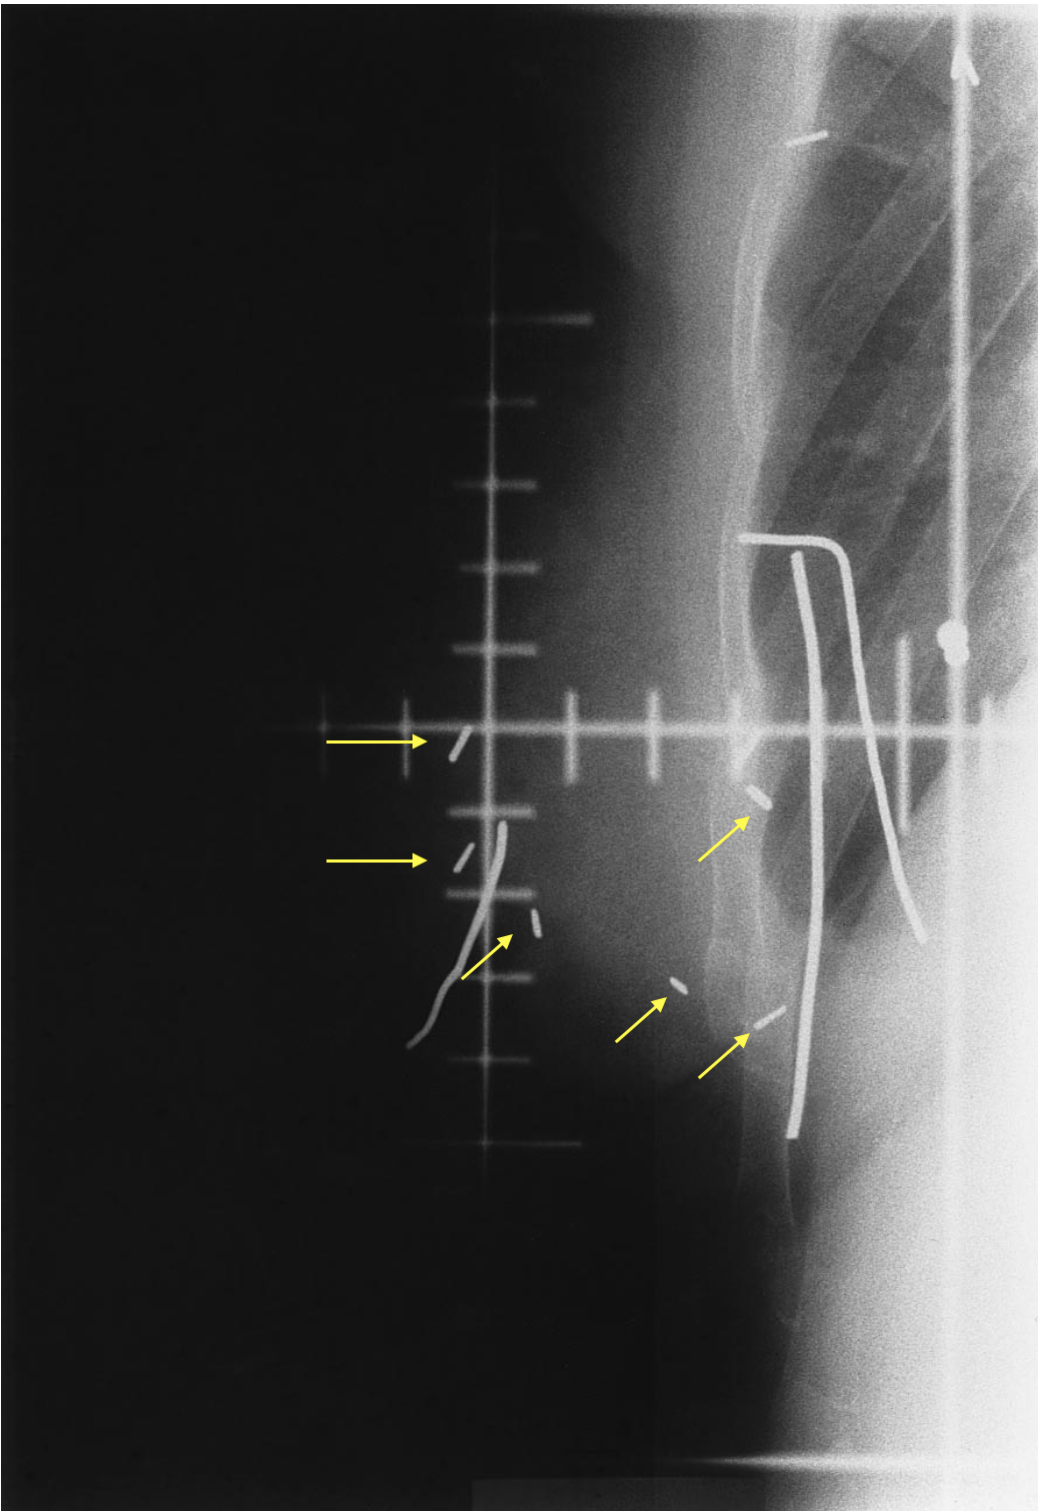
\includegraphics[height=0.3\textheight]{../figs/literature_review/imaging_of_fiducal_clips_in_phantom_breast.png}
        \caption{Imaging of Fiducial Clips in Phantom Breast. Yellow arrows indicate fiducial clips placed around tumor cavity. Adapted from \cite{RefWorks:RefID:178-krawczyk1994importance}.}
        \label{fig:literatureReview:imaging_of_fiducal_clips_in_phantom_breast}
\end{figure}

\subsection{Seroma Formation\label{sec:literatureReview:seromaFormation}}
\hl{Add more here about seromas}
Review of current accepted...\cite{RefWorks:RefID:25-acree2022review} has great stats on this (see Figure~\ref{fig:literatureReview:seromaFormationStats}).
\begin{figure}[h]
        \centering
        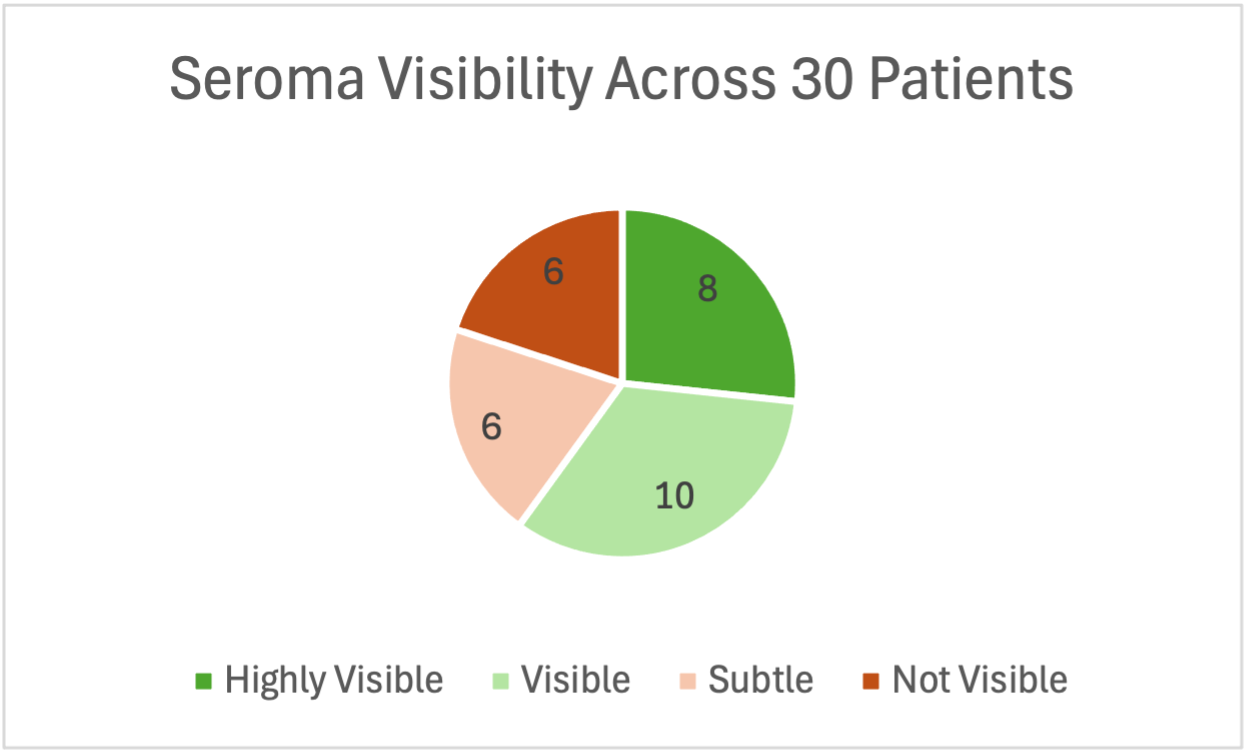
\includegraphics[width=0.7\textwidth]{../figs/literature_review/seroma_visibility_study_results.png}
        \caption{Statistics on Seroma Formation from \cite{RefWorks:RefID:25-acree2022review}.}
        \label{fig:literatureReview:seromaFormationStats}
\end{figure}

Using seroma formation to mark the tumor bed for radiation therapy involves outlining the seroma that forms following a lumpectomy procedure~\cite{RefWorks:RefID:25-acree2022review}.

\subsection{Implantable Devices\label{sec:literatureReview:implantableDevices}}
Lastly, implantable devices can be used to mark the tumor bed. One example is BioZorb (Hologic) which is a 3-dimensional coil-like structure with titanium clips embedded. This device is implanted into the tumor cavity following a lumpectomy procedure and improves on titanium clips alone by creating a 3D outline of the tumor bed. BioZorb was also designed to be reabsorbed into the body within a year~\cite{RefWorks:RefID:25-acree2022review}. BioZorb is shown below in Figure~\ref{fig:literatureReview:biozorb_implant}.
\begin{figure}[h!]
        \begin{minipage}{0.92\textwidth}
                \centering
                \begin{subfigure}[b]{0.9\textwidth}
                        \centering
                        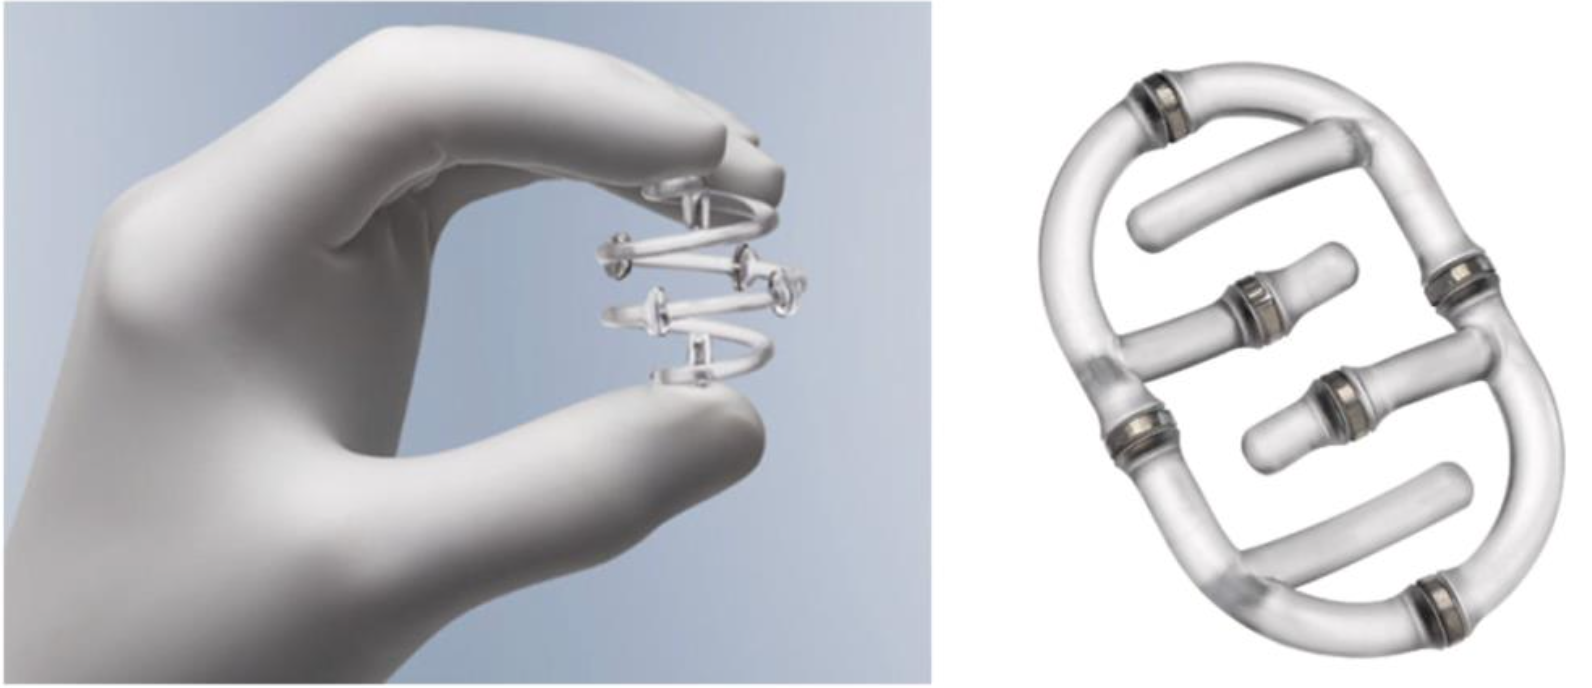
\includegraphics[width=\textwidth]{../figs/literature_review/BioZorb_physically.png}
                        \caption{BioZorb physically (top).}
                        \label{fig:literatureReview:biozorb_physically}
                \end{subfigure}

                \vspace{1em} % optional space between images

                \begin{subfigure}[b]{0.9\textwidth}
                        \centering
                        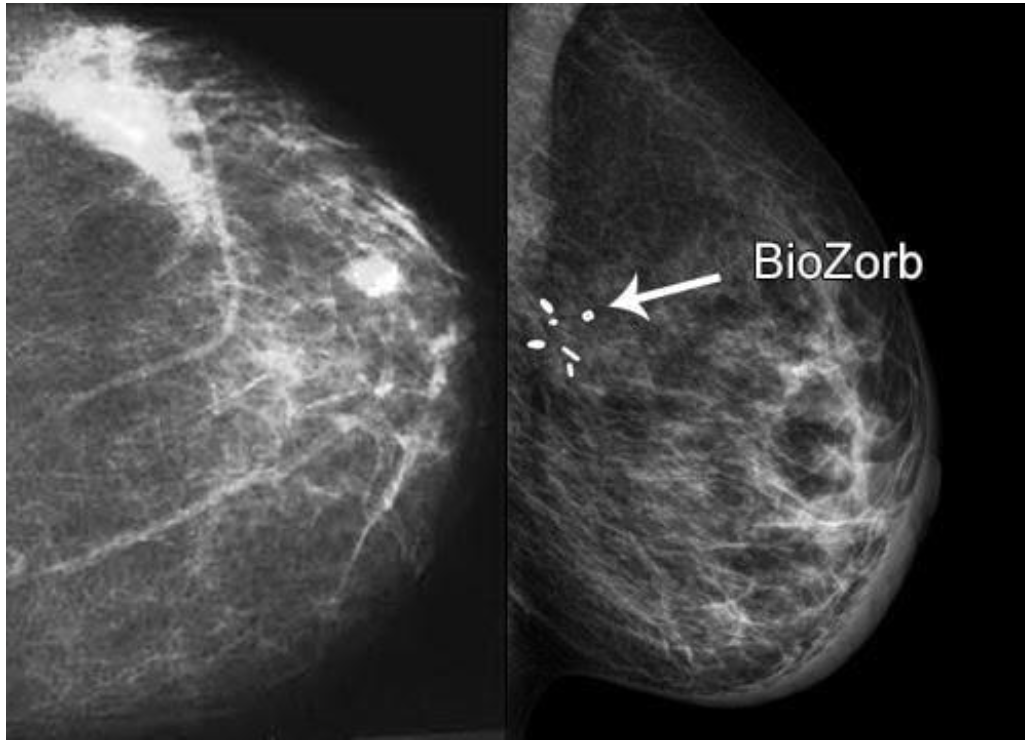
\includegraphics[width=\textwidth]{../figs/literature_review/BioZorb_in_imaging.png}
                        \caption{BioZorb in imaging.}
                        \label{fig:literatureReview:biozorb_in_imaging}
                \end{subfigure}
        \end{minipage}
        \caption{BioZorb, an implantable device to assist with TB delineation~\cite{RefWorks:RefID:370-einsteinisaac}.}
        \label{fig:literatureReview:biozorb_implant}
\end{figure}

\subsection{Veraform\label{sec:literatureReview:veraform}}
A newer implantable device is Veraform, a continuously radiographically opaque filament that is stitched around the tumor cavity. By being malleable and sewn in place, this device addresses space limitations and migration issues present in other devices~\cite{RefWorks:RefID:344-mitchell2019adaptable}. A simulation showing Veraform in use is shown below in Figure~\ref{fig:literatureReview:veraform_implant}.
\begin{figure}[h!]
        \centering
        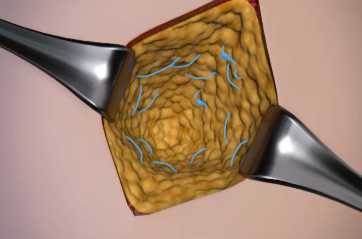
\includegraphics[width=0.6\textwidth]{../figs/literature_review/veraform_implant.png}
        \caption{Veraform, an implantable device to assist with TB delineation~\cite{RefWorks:RefID:344-mitchell2019adaptable}.}
        \label{fig:literatureReview:veraform_implant}
\end{figure}

\subsection{Challenges with Current Devices and Methods\label{sec:introduction:motivation:challengeswithcurrentdevicesandmethods}}
\hl{See if this could use more detail.}
\subsubsection{Challenges with Fiducial Markers\label{sec:introduction:motivation:challengeswithcurrentdevicesandmethods:challengeswithfiducialmarkers}}
There are many challenges and inaccuracies that can result from using fiducial markers or surgical clips to create a TB volume. They provide single points of reference which can lead to inaccurate boundaries being drawn, there is no standardized recommendation of how many clips should be used, and clips can migrate over time leading to inaccurate TB localization~\cite{RefWorks:RefID:344-mitchell2019adaptable}. Migration is especially common when patients undergo oncoplastic reconstruction surgery following the lumpectomy procedure. In 2022, it was found the 30,000 breast-conserving therapy patients annually undergo oncoplastic reconstruction surgery~\cite{RefWorks:RefID:25-acree2022review}.

Another concern of surgical clips or fiducial markers is if a re-excision is required. This is when a margin of tissue removed during the lumpectomy is found to contain cancerous cells. When this is the case, a large enough margin surrounding the tumor was not removed, and a re-excision has to be made to remove additional margins. When markers are placed initially, these re-excisions can impact the accuracy of the initial marker placement. It was found that 10\% to 20\% of patients undergoing breast-conserving surgery require a re-excision~\cite{RefWorks:RefID:25-acree2022review}.

\subsubsection{Challenges with Seroma Formation\label{sec:introduction:motivation:challengeswithcurrentdevicesandmethods:challengeswithseromaformation}}
\hl{Show change in seroma over time visual.\\}

Utilizing seroma formation can be unreliable, as the seroma may not always be localized to the tumor bed, relies on the excision closure method, and time elapsed after surgery\cite{RefWorks:RefID:25-acree2022review}. A seroma may represent the tumor bed, part of the tumor bed, or the entire area in which surgery was performed~\cite{RefWorks:RefID:344-mitchell2019adaptable}.

\subsubsection{Challenges with Biozorb}
Biozorb was found to provide limited value to patients relative to its high cost~\cite{RefWorks:RefID:344-mitchell2019adaptable}. Additionally, Biozorb was also recalled due to patient discomfort, seroma formation, device migration, and failures to resorb into the body in the designated timeframe~\cite{RefWorks:RefID:296-2024hologic},~\cite{RefWorks:RefID:28-nudelunited}.
